% SAIGE-slim: what's new, for people who want to run it
% Consortium presentation, 2026-10-01.  SKAT-O arm only.
%
% Build: pdflatex saige-slim-consortium-2026-10-01.tex   (twice)
% If metropolis is unavailable: swap \usetheme{metropolis} for \usetheme{default}
\documentclass[aspectratio=169,11pt]{beamer}
\usetheme{metropolis}
\usepackage{booktabs}
\usepackage{xcolor}
\usepackage{graphicx}
\definecolor{acc}{HTML}{1F5673}
\definecolor{good}{HTML}{2E6F40}
\setbeamercolor{frametitle}{bg=acc}
\newcommand{\win}[1]{\textcolor{good}{\textbf{#1}}}

\title{SAIGE-slim: faster, smaller, and easier to run}
\subtitle{Gene-based (SKAT-O) and single-variant tests --- what's new and what to switch on}
\date{1 October 2026}
\author{Duncan Palmer}

\begin{document}
\maketitle

% ---------------------------------------------------------------------------
\begin{frame}{The short version}
Same tests. Same answers. Considerably less compute and far less data movement.

\medskip
\begin{itemize}
  \item \win{PLINK 2 (PGEN) input} at every step --- and for rare coding variants
        the files are \emph{dramatically} smaller.
  \item \win{$2.1\times$ faster} gene-based runs from a single change to the
        SKAT-O p-value kernel.
  \item \win{Multi-threaded} step 2, and \win{many phenotypes / many null models
        in one pass} --- so the genotypes are read once, not once per trait.
  \item \win{Two default flags worth turning off} --- one of them $1.23\times$
        faster \emph{and} statistically cleaner.
  \item \win{It refuses bad runs up front} instead of burning a day and
        producing a model you can't use.
\end{itemize}

\medskip
\textbf{Two kinds of change, and the difference matters.} The engineering --- the
PGEN reader, sparse decode, threading, carrier-space gene tests --- is gated on
\textbf{byte-identical output} against a committed reference set, so none of it
can move a result. The statistical changes (the SKAT-O kernel, and the two flags)
\emph{do} change numbers, deliberately and for the better --- and each has a flag
that recovers the old behaviour exactly, so you can verify the difference
yourself rather than take it on trust.
\end{frame}

% ---------------------------------------------------------------------------
\begin{frame}{PGEN: the one that surprised us}
Real numbers, AoU chromosome 20 exome, 79,956 samples, coding variants only ---
on a file \textbf{already filtered} to AF\,$<$\,1\,\% with popmax\,$<$\,1\,\%, i.e.\
rare in \emph{every} population:

\medskip
\begin{center}
\begin{tabular}{lrr}
\toprule
 & size & \\
\midrule
Full \texttt{.bed} (all 307,558 variants) & 5.73 GiB & \\
Coding subset \texttt{.bed} (119,863 variants) & 2.30 GiB & \\
\textbf{Coding subset \texttt{.pgen}} & \win{13 MB} & \win{$\sim$180$\times$ smaller} \\
\quad {\footnotesize + \texttt{.pvar} 4.1 MB, \texttt{.psam} 859 KB} & & \\
\bottomrule
\end{tabular}
\end{center}

\medskip
\textbf{Why it is so extreme.} About 90\,\% of coding variants are ultra-rare. A
\texttt{.bed} record is a fixed 2 bits per sample --- here 19,989 bytes per
variant --- most of it spent saying \emph{``almost nobody carries this''}. PGEN
stores the carriers instead, so the file scales with signal rather than with
cohort size.

\medskip
\textbf{The ratio is set by how rare your variants are}, which is why it is worth
filtering before you store:

\medskip
\begin{center}\small
\begin{tabular}{lr}
\toprule
Unfiltered whole chromosome {\footnotesize (simulated, $N=50{,}000$)} & $6.4\times$ \\
\quad {\footnotesize 2509\,MB \texttt{.bed} $\to$ 389\,MB \texttt{.pgen}} & \\
Coding \emph{and} pre-filtered to AF\,$<$\,1\,\% {\footnotesize (AoU, above)} & \win{$\sim$180$\times$} \\
\bottomrule
\end{tabular}
\end{center}

\medskip
\textbf{Read the two honestly.} $6.4\times$ is what you get on an unfiltered
file; $\sim$180$\times$ needs a file already restricted to rare variants, which
is what a rare-variant analysis uses but is not a general bed-to-pgen ratio.
Expect somewhere between the two, nearer the top end the harder you filter.
{\footnotesize (The AoU \texttt{.bed} sizes are computed exactly from the record
size and variant count, against a measured \texttt{.pgen}; same variant set both
sides.)}
\end{frame}

\begin{frame}{Why that matters more than any decode benchmark}
\begin{center}
\emph{Our published speedups are a lower bound.}
\end{center}

\medskip
On a dsub/batch workflow the worker \textbf{localizes the whole genotype file from
object storage before your script starts}. That time appears in your wall clock
and in your bill, and in \emph{none} of the decode benchmarks on the next slide.

\medskip
\begin{itemize}
  \item 2.3\,GiB $\to$ 13\,MB changes localization from minutes to seconds, per
        task, across every trait and every chromosome.
  \item It also cuts egress, storage and the time to stage a cohort for a new
        analysis.
\end{itemize}

\medskip
PGEN also needs no special flags here --- upstream 1.4.2 refuses PGEN without
\texttt{--AlleleOrder=ref-first}; our reader does not.
\end{frame}

\begin{frame}{Sparse decode: up to $10\times$ on a rare-variant scan}
PGEN already stores a rare variant as a list of its carriers. We now \emph{read}
it that way --- doing the per-variant work over the carriers instead of over the
whole cohort. The rarer the variant, the bigger the saving.

\medskip
\begin{center}
\begin{tabular}{lr}
\toprule
\textbf{On a file filtered to MAF\,$<$\,1\,\%} --- i.e.\ a rare coding analysis & \\
\quad quantitative trait & \win{$10.4\times$} \\
\quad binary trait, Firth off & \win{$6.1\times$} \\
\addlinespace
\textbf{Unfiltered, whole-exome} & \\
\quad quantitative & \win{$1.87\times$} \\
\quad binary & $1.21\times$ \\
\bottomrule
\end{tabular}
\end{center}

\medskip
\textbf{And it compounds with the file size.} The same MAF filter that shrinks
the \texttt{.pgen} to megabytes is what makes the sparse decode pay best --- you
move $\sim$180$\times$ less data \emph{and} scan it up to $10\times$ faster. Those
are the same analysis, not two different ones.

\medskip
{\footnotesize Single-variant scan, $N=50{,}000$, 1 thread, measured against our
own dense-read path (which is what upstream does). Every output byte-identical;
\texttt{SAIGE\_PGEN\_SPARSE=0} is the kill switch.}
\end{frame}

\begin{frame}{Where the sparse decode does \emph{not} help --- and why that's fine}
The same technique on the gene-test path gives much less:

\medskip
\begin{center}
\begin{tabular}{lr}
\toprule
Burden gene tests & $1.56\times$ \\
SKAT-O gene tests & $1.13\times$ \\
\bottomrule
\end{tabular}
\end{center}

\medskip
\textbf{Because that is not where a SKAT-O run spends its time.} Gene-test cost
sits in the p-value kernel, not in reading genotypes --- which is exactly what
the \win{$2.14\times$} on the next slide addresses.

\medskip
\begin{center}
\emph{Two bottlenecks, two fixes:} \\[0.4em]
rare-variant scans were I/O-and-decode bound $\rightarrow$ sparse decode \\
SKAT-O gene tests were kernel bound $\rightarrow$ new p-value method
\end{center}

\medskip
If you run both arms, you get both.
\end{frame}

\begin{frame}{Where the compute savings come from}
\begin{center}
\begin{tabular}{lr}
\toprule
Change & Measured \\
\midrule
SKAT-O p-value kernel: closed form above threshold, & \win{$2.14\times$} whole run \\
\quad exact method below it {\footnotesize ($N=50{,}000$)} & {\footnotesize 207\,s $\to$ 96.7\,s} \\
\addlinespace
Gene-test genotype handling in carrier space & \win{$\sim$40\,\% less peak RAM} \\
 & {\footnotesize 874\,MB $\to$ 520\,MB} \\
\addlinespace
Identical gene-test cells evaluated once & reported per run \\
\addlinespace
Turning off approximate-Firth effect sizes & \win{$\sim2\times$} on binary \\
 & \quad single-variant scans \\
\addlinespace
Multi-threading step 2 \texttt{--nThreads} & scales to $\sim$4 threads \\
\bottomrule
\end{tabular}
\end{center}

\medskip
{\footnotesize Each gated on byte-identical output. The SKAT-O kernel change also
\emph{improves} accuracy below $p\sim10^{-5}$, where the shipped method is
unreliable --- so this is not a speed/accuracy trade.}
\end{frame}

% ---------------------------------------------------------------------------
\begin{frame}{Two flags to turn off --- and why}
\textbf{1.\quad\texttt{--is\_Firth\_beta=FALSE}}
\begin{itemize}
  \item Approximate-Firth is \textbf{56\,\% of CPU} on a binary single-variant
        scan (17.5\,ms per marker it fires on).
  \item \textbf{This reaches your gene-test runs too.} A SKAT-O run
        (\texttt{--r.corr=0}) always emits single-variant results for the markers
        in each group, so it contains a single-variant scan whether you asked for
        one or not.
  \item It refines \textbf{effect-size estimates only}. Your p-values do not
        depend on it.
  \item Already our default; upstream pipeline wrappers commonly set it on.
  \item \textbf{It also eats the sparse-decode gain}: on a MAF\,$<$\,1\,\% file a
        binary scan is $6.1\times$ faster with Firth off and only $2.8\times$ with
        it on. The two savings compound.
\end{itemize}

\medskip
\textbf{2.\quad\texttt{--is\_fastTest=FALSE}}
\begin{itemize}
  \item \texttt{fastTest} is a two-pass scheme: a cheap pass, then anything below
        \texttt{--pval\_cutoff\_for\_fastTest} re-tested properly, and the second
        result reported.
  \item So \textbf{a reported p-value near the cutoff depends on the cutoff}.
  \item \alert{And measured, it is a net LOSS to leave on}: $1.23\times$ faster
        with it off, because when many cells fall below the re-test cutoff you pay
        for \emph{both} passes.
  \item So this is not a speed-versus-rigour trade --- off is both.
\end{itemize}

\medskip
\begin{center}
Both off is what we run in production.
\end{center}
\end{frame}

% ---------------------------------------------------------------------------
\begin{frame}{New: read the genotypes once, not once per trait}
\begin{itemize}
  \item \win{\texttt{--nThreads}} threads step 2 in-process --- the marker scan
        and both gene-test paths --- \textbf{byte-identical at any thread count},
        and the run \emph{reports} the count it used.
  \item \win{Many phenotypes in one step-1 process}
        (\texttt{--phenoCol=y1,y2,\dots}), writing per-phenotype outputs plus a
        manifest that step 2 consumes. Each output is byte-identical to a
        standalone run's.
  \item \win{Many null models in one step-2 genotype pass}, on both the
        single-variant and gene-test paths. For a consortium running dozens of
        traits on the same cohort, \textbf{this amortises the expensive part}
        across all of them.
\end{itemize}

\medskip
{\footnotesize One constraint worth knowing: a sparse-GRM step-1 fit is
single-threaded whatever \texttt{--nThreads} says --- so size those machines for
RAM, not cores.}
\end{frame}

% ---------------------------------------------------------------------------
\begin{frame}{It tells you no \emph{before} you spend the compute}
Five eligibility checks, run before and after the null fit, each with a flag and
a sensible default:

\medskip
\begin{center}\small
\begin{tabular}{ll}
\toprule
Check & Default \\
\midrule
Minimum case count \texttt{--minCaseCount} & 100 \\
Minimum covariate cell count & 10 \\
Quasi-separation, as a \emph{fraction} of samples & 2\,\% \\
Convergence of the null fit & refuse \\
Minimum sample count & off \\
\bottomrule
\end{tabular}
\end{center}

\medskip
A binary trait with too few cases, a covariate level with no cases, or a fit that
did not converge is \textbf{refused with a named reason} --- not silently saved as
a model you will analyse for a week and then distrust.

\medskip
{\footnotesize In our own production refit this caught 21 of 164 binary fits that
had quietly failed to converge. Thresholds are flags: set them to your own study's
policy.}
\end{frame}

\begin{frame}{And when something does go wrong, it says so}
Alongside the results, each run writes small companion files:

\medskip
\begin{center}\small
\begin{tabular}{ll}
\toprule
\texttt{.chrStatus.txt} & requested / failed / refused / skipped, per chromosome \\
\texttt{.skatoMethod.txt} & which p-value method each cell used \\
\texttt{.skatFailures.txt} & cells where the kernel failed (rows stay \texttt{NA}) \\
\texttt{.pooledTests.txt} & how each pooled row was combined \\
\texttt{.spaFallbacks.txt} & any test that fell back, and why \\
\bottomrule
\end{tabular}
\end{center}

\medskip
\begin{itemize}
  \item \textbf{A lost chromosome is visible} rather than a quietly short results
        file.
  \item \textbf{A restart resumes the \emph{results} exactly.} Chunk byte offsets
        are recorded for the results file and the single-variant file; a restart
        truncates to them and reproduces a complete run byte-for-byte. It no
        longer duplicates rows or re-runs a completed chunk.
  \item \alert{But the companion files above are written at end of run and
        \emph{overwritten}, so after a restart they describe only the resumed
        portion.} If you restart, treat them as partial --- or re-run the prefix
        to regenerate them. Known limitation, not yet fixed.
  \item A repeated sample ID is refused at every step rather than silently treated
        as one individual.
\end{itemize}
\end{frame}

% ---------------------------------------------------------------------------
\begin{frame}{Getting it}
\begin{itemize}
  \item \textbf{Docker image}, built from a pinned lockfile; reproduces a
        reference output byte-identically on Linux. No build required.
  \item \textbf{Drop-in}: same step 0 / step 1 / step 2 structure, same flags,
        plus PGEN input and the new options above.
  \item \textbf{Steps covered}: sparse GRM, null GLMM, single-variant and
        gene-based (SKAT-O) tests. Binary and quantitative traits.
  \item Continuous integration on every change, against 170 committed reference
        outputs and $\sim$7{,}000 assertions.
\end{itemize}

\medskip
\textbf{One gotcha to carry away:} \texttt{--relatednessCutoff} must \emph{match}
between steps. Nothing upstream enforces it, and a mismatch silently tests
against a variance ratio that describes a different GRM. Our wrapper requires it
explicitly.
\end{frame}

\begin{frame}{Same answers: gene tests against upstream, $N=50{,}000$}
\begin{center}
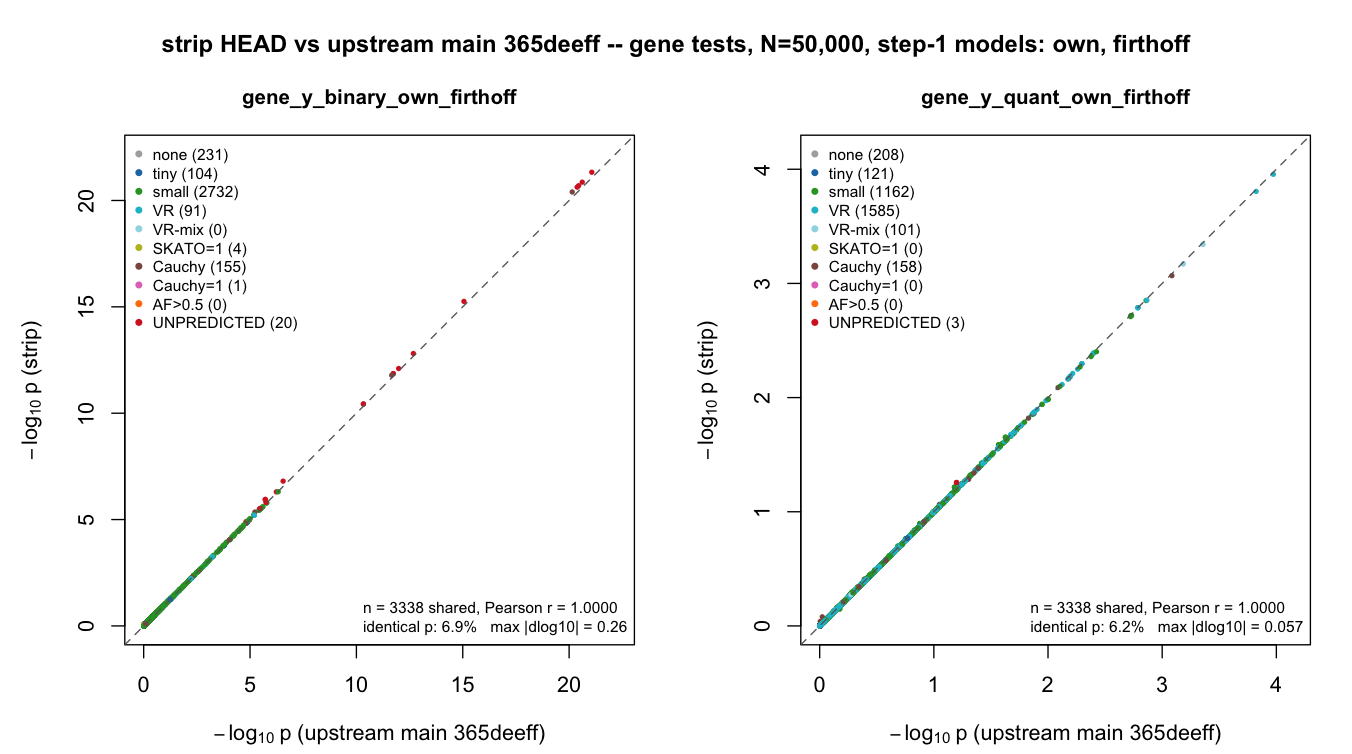
\includegraphics[width=0.92\textwidth]{figs/gene_own_firthoff.png}
\end{center}
\vspace{-0.3em}
{\footnotesize 3,338 shared gene-test cells per trait. Pearson $r$ on $-\log_{10}p$
= \textbf{0.99997} (binary), \textbf{1.0000} (quantitative).}
\end{frame}

\begin{frame}{What the handful of departures are}
Every point off the diagonal is attributed, not tolerated. The comparator tags each
one with a cause and reconciles it; \texttt{UNPREDICTED} means ``stop and explain''.

\medskip
\textbf{The 20 binary departures are \emph{us} correcting \emph{upstream}.}
LEDGER \#104/\#105: upstream's binary burden variance is inflated. Re-running our
code with those fixes reverted gives:

\medskip
\begin{center}\small
\begin{tabular}{lrr}
\toprule
 & \texttt{UNPREDICTED} & max $|\Delta\log_{10}p|$ \\
\midrule
Our build, binary gene tests & 20 & 0.26 \\
\quad with the fixes reverted & \win{0} & \win{0.018} \\
\bottomrule
\end{tabular}
\end{center}

\medskip
So the agreement is exact once the deliberate corrections are removed --- which is
the strongest form of this claim available: we can reproduce upstream's numbers on
demand, and we can say precisely why we don't.

\medskip
{\footnotesize Comparison predates the new SKAT-O kernel, so it isolates the
\emph{engineering}. The kernel change is covered separately --- it moves p-values
on purpose, below $10^{-5}$ and above $0.05$.}
\end{frame}

\begin{frame}{Measured: versus your current run}
One fixture, one build, flags only --- the SKAT-O kernel is flag-controlled, so
the ``old kernel'' arm reproduces upstream's kernel byte for byte and every term
below is isolated rather than confounded.

\medskip
{\footnotesize Simulated chr20, $N=50{,}000$, binary trait, 6 masks $\times$ 3 max MAFs,
single-variant results on, 1 thread. Genotype localization excluded.}

\medskip
\begin{center}\small
\begin{tabular}{llr}
\toprule
\textbf{Your current run} & bed, Firth on, fastTest on, old kernel & 218.4\,s \\
\textbf{Recommended} & pgen, Firth off, fastTest off, new kernel & \win{77.9\,s} \\
\midrule
 & \textbf{speedup} & \win{$\mathbf{2.80\times}$} \\
\bottomrule
\end{tabular}
\end{center}

\medskip
Each term measured separately, same way:

\medskip
\begin{center}\small
\begin{tabular}{lr}
\toprule
New SKAT-O p-value kernel & \win{$2.04\times$} \\
\texttt{--is\_fastTest=FALSE} & \win{$1.23\times$} \\
PGEN + sparse decode & \win{$1.13\times$} \\
\texttt{--is\_Firth\_beta=FALSE} & $1.005\times$ {\footnotesize --- nothing, see note} \\
\bottomrule
\end{tabular}
\end{center}

\medskip
Before \texttt{--nThreads} (scales to $\sim$4 threads) and before the
localization saving, 2.3\,GiB $\to$ 13\,MB per task.
\end{frame}

\begin{frame}{Two things that measurement changed}
\textbf{1.\quad\texttt{fastTest} off is \emph{faster}, not a trade.}
We expected turning it off to cost speed --- it buys a cheap first pass, after
all. Measured, it is a \win{$1.23\times$ net loss} to leave on: when a large share
of cells fall below its $p=0.05$ re-test cutoff you pay for \emph{both} passes.

\medskip
\begin{center}
So \texttt{--is\_fastTest=FALSE} is faster \emph{and} removes a cutoff-dependent
p-value. Not a trade at all.
\end{center}

\medskip
\textbf{2.\quad Firth costs nothing on a gene-test run.}
The $56\,\%$-of-CPU figure is a genome-wide \emph{scan} number and does not
transfer: inside gene tests the single-variant markers are few and rare, so Firth
barely fires. It did fire here --- 1069 single-variant rows moved --- and the
gene-level results were \textbf{byte-identical}, confirming it touches effect
sizes only.

\medskip
\alert{So gene-level \texttt{BETA\_Burden} is never Firth-corrected,} whichever
way you set the flag. Turn it off for your variant scans; for gene tests it costs
you nothing either way.

\medskip
{\footnotesize Repeat spread across arms: 1.9--3.5\,\%, so the $1.005\times$ is a
real null rather than an effect hidden by noise. The decomposition reconciles two
ways ($2.48\times1.13$ and $1.375\times2.04$, both giving $2.80$).}
\end{frame}

\begin{frame}[standout]
In one line

\medskip
{\large
Gigabytes become megabytes, \\
gene tests run twice as fast, \\
and the genotypes are read once for all your traits. \\[1.2em]
\normalsize Same answers --- byte-identical output is the gate.
}
\end{frame}

\end{document}
